\section{Overview of the Recommenders Repository}

The repository is open-source under the MIT License and contributions that follow the guidelines are encouraged.  
The development follows standard Github practices such as issues, milestones and pull requests.

All the algorithms and utilities have been written in the Python programming language and the demostrations are 
in the form of Jupyter notebooks \cite{jupyter}.

The platforms supported are Linux and Windows, on a local computer, on premises, or on the Azure Cloud \cite{azure}, depending on availability of resources.
Some of the algorithms can take advantage of GPU resources if available and some others require a Spark environment \cite{spark}.

\begin{figure}
  \centering
  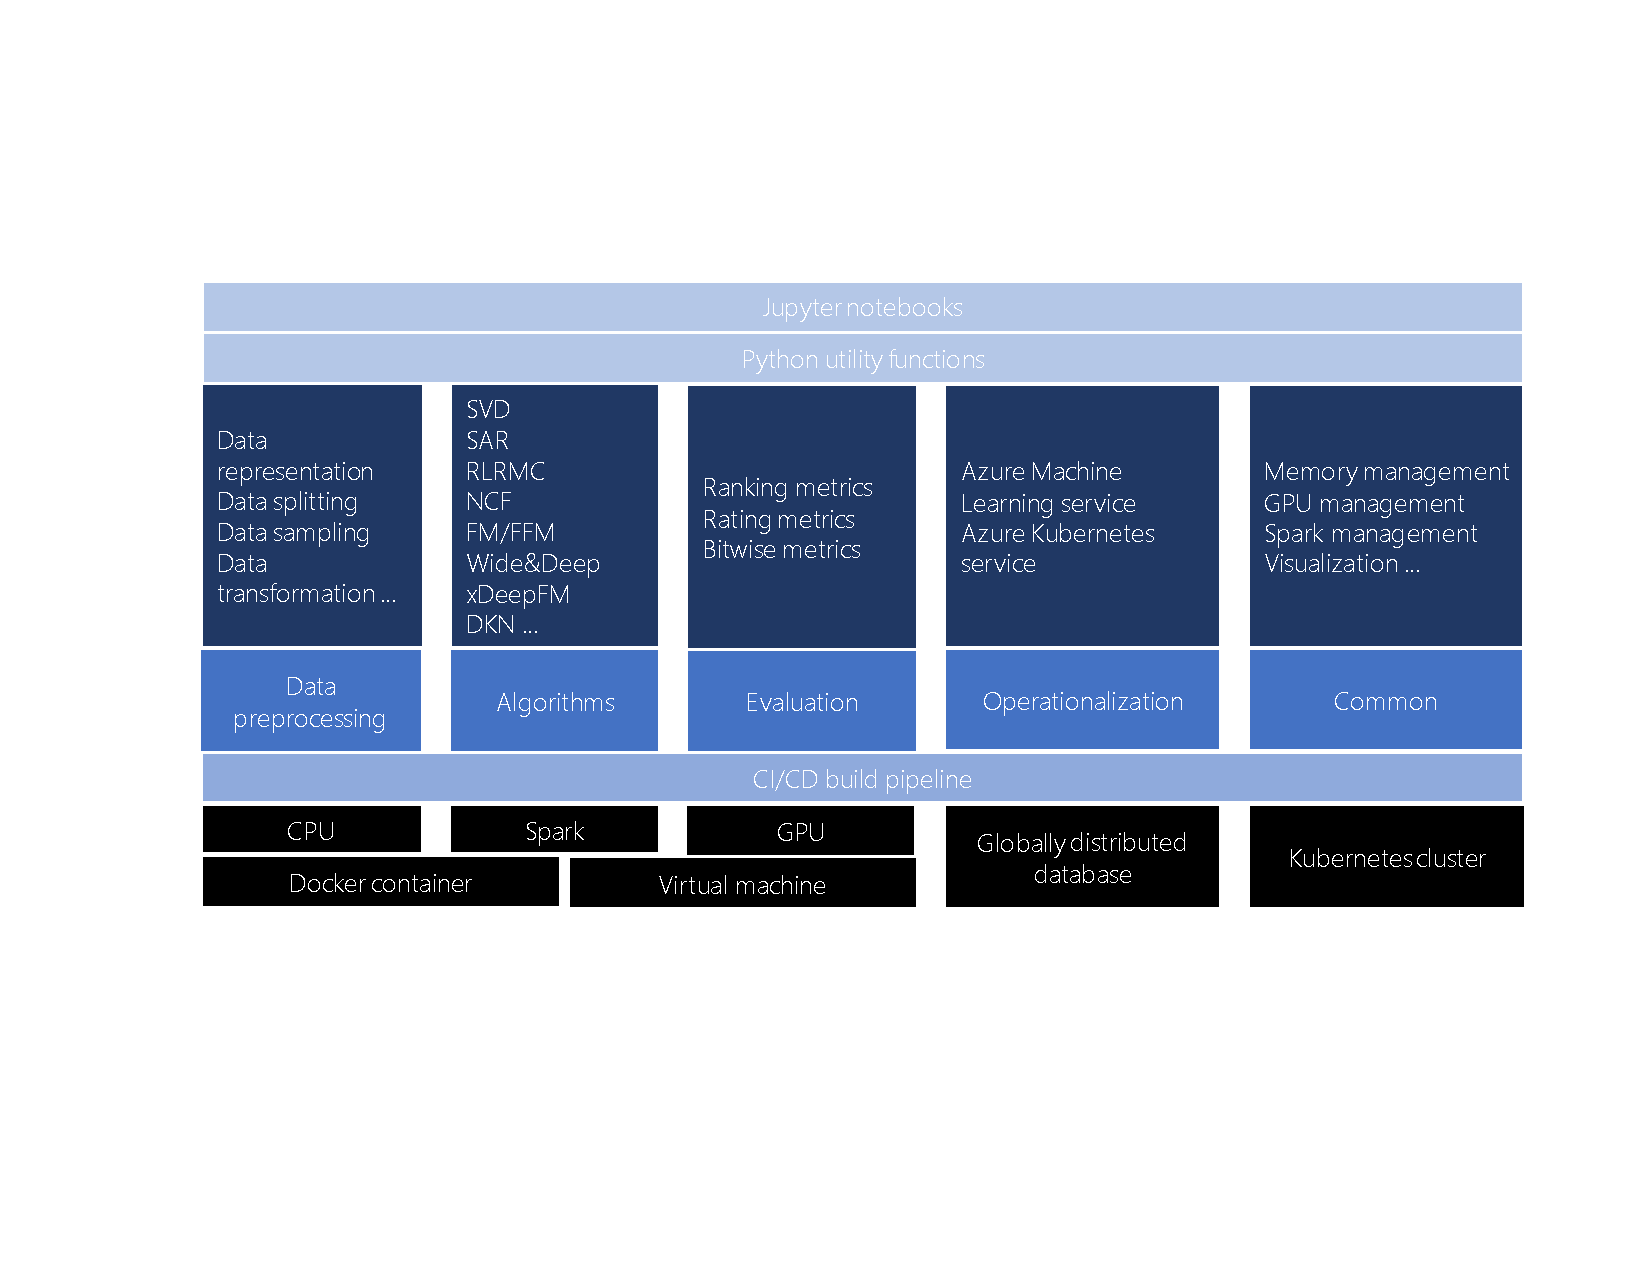
\includegraphics[width=\textwidth,keepaspectratio]{platform_diagram_crop.pdf}
  \caption{Microsoft Recommenders structure diagram. Layers from the bottom to the top support the underlying infrastructure, build pipeline, recommendation pipeline tasks, and example notebooks and utility functions.}
\end{figure}

Microsoft-Recommenders is based on best practices for building recommendation systems, which have been learned from application with production-ready systems.
As a consequence, we have followed an {\em end-to-end} approach, which is not limited to just the training of an algorithm, but encompasses the following components, typical in a recommendation pipeline:

\begin{itemize}
\item Data preparation: Preparing and loading data for each recommender algorithm
\item Model: Building models using various classical and deep learning recommender algorithms such as Alternating Least Squares (ALS) \cite{koren2009matrix} or eXtreme Deep Factorization Machines (xDeepFM) \cite{lian2018xdeepfm}.
\item Evaluate: Evaluating algorithms with offline metrics
\item Model Select and Optimize: Tuning and optimizing hyperparameters for recommender models
\item Operationalize: Operationalizing models in a production environment on Azure
\end{itemize}

Several utilities are provided in the 
reco utils folder\footnote{\url{https://github.com/microsoft/recommenders/blob/master/reco_utils}} 
to support common tasks such as loading datasets in the format expected by 
different algorithms, evaluating model outputs, and splitting training/test data. 
Implementations of several state-of-the-art algorithms are provided for self-study and 
customization in one's own applications.

